\section{Resolving Compton interactions}
\label{sec.comp}

Photoelectric interactions are a relatively small fraction of the total number of interactions in LXe (22\%) as well as in SSDs (for example, 33\% in LSO). The bulk of Compton interactions can result either in contained (when the scatter gamma produces a cascade that does not escape the detector) or non contained events. Non contained events do not deposit the full energy of the gamma in the detector and can be rejected. However, the large fraction of contained Compton events (60\% for the LXSC and larger for denser SSDs, such as LSO) introduce a significant distortion of the position in the case of conventional SSDs. Recall that conventional SSDs do not measure the $z$~(longitudinal) coordinate, introducing parallax errors. In addition, when a multiple-site Compton interaction occur in the detector, the transverse ($x,y$) coordinates are distorted, since the system only measures the average coordinate. 

Instead, in the LXSC, multiple-site hits could be identified (the system measures true 3D points) and separated to a distance of the order of the detector pitch. This capability of separating photoelectric and Compton events in the LXSC can be further exploited in the case of 2-site Compton interactions. Resolving the position and the energy of both gammas with good resolution would allow the LXSC to operate as a {\em Compton Telescope}, taking advantage of Compton kinematics to further restrict the point of emission of the photons. 


\begin{figure}[!htb]
	\centering
	\subfloat[Compton event with 2 clusters]{
		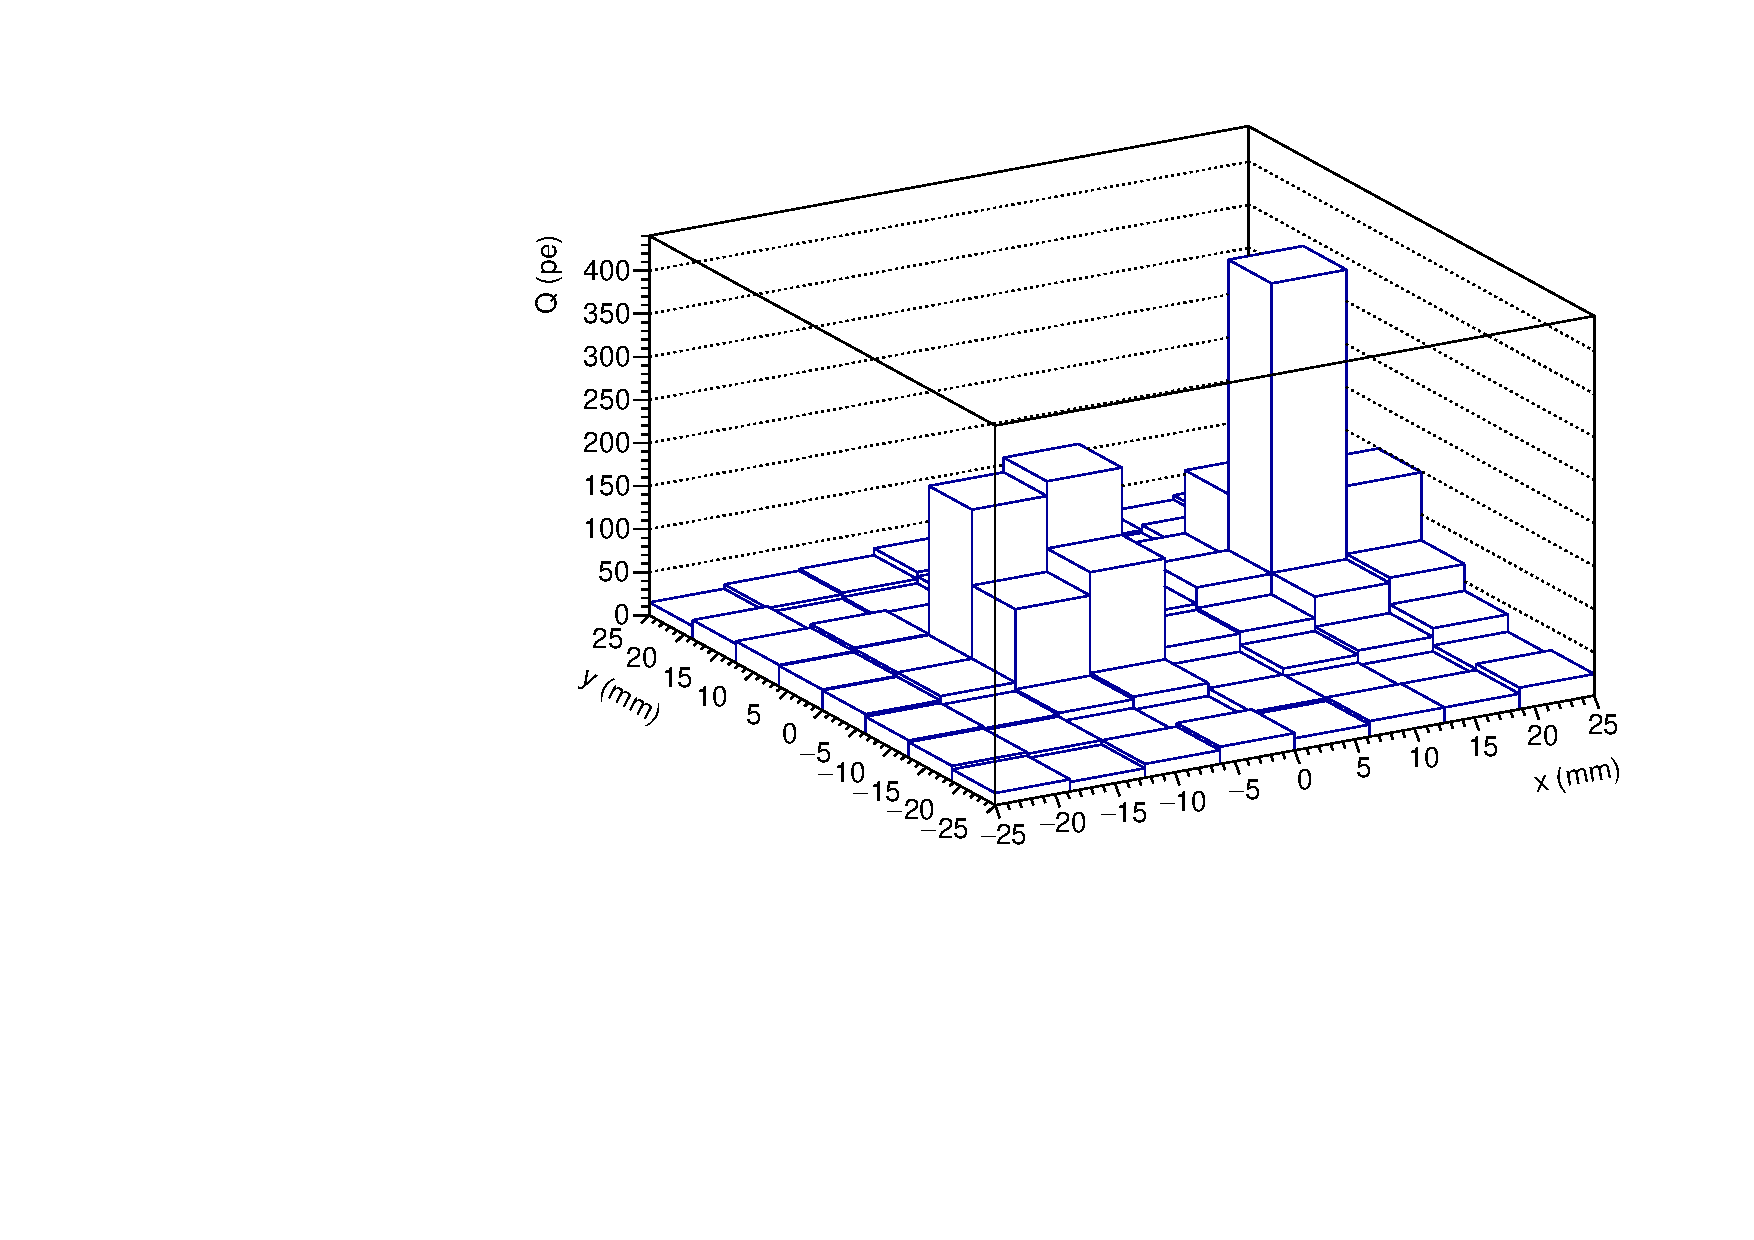
\includegraphics[width=.5\textwidth]{img/compton_2cluster.pdf}
		\label{fig.compton1}
	}
	\subfloat[Compton event with 1 cluster]{
		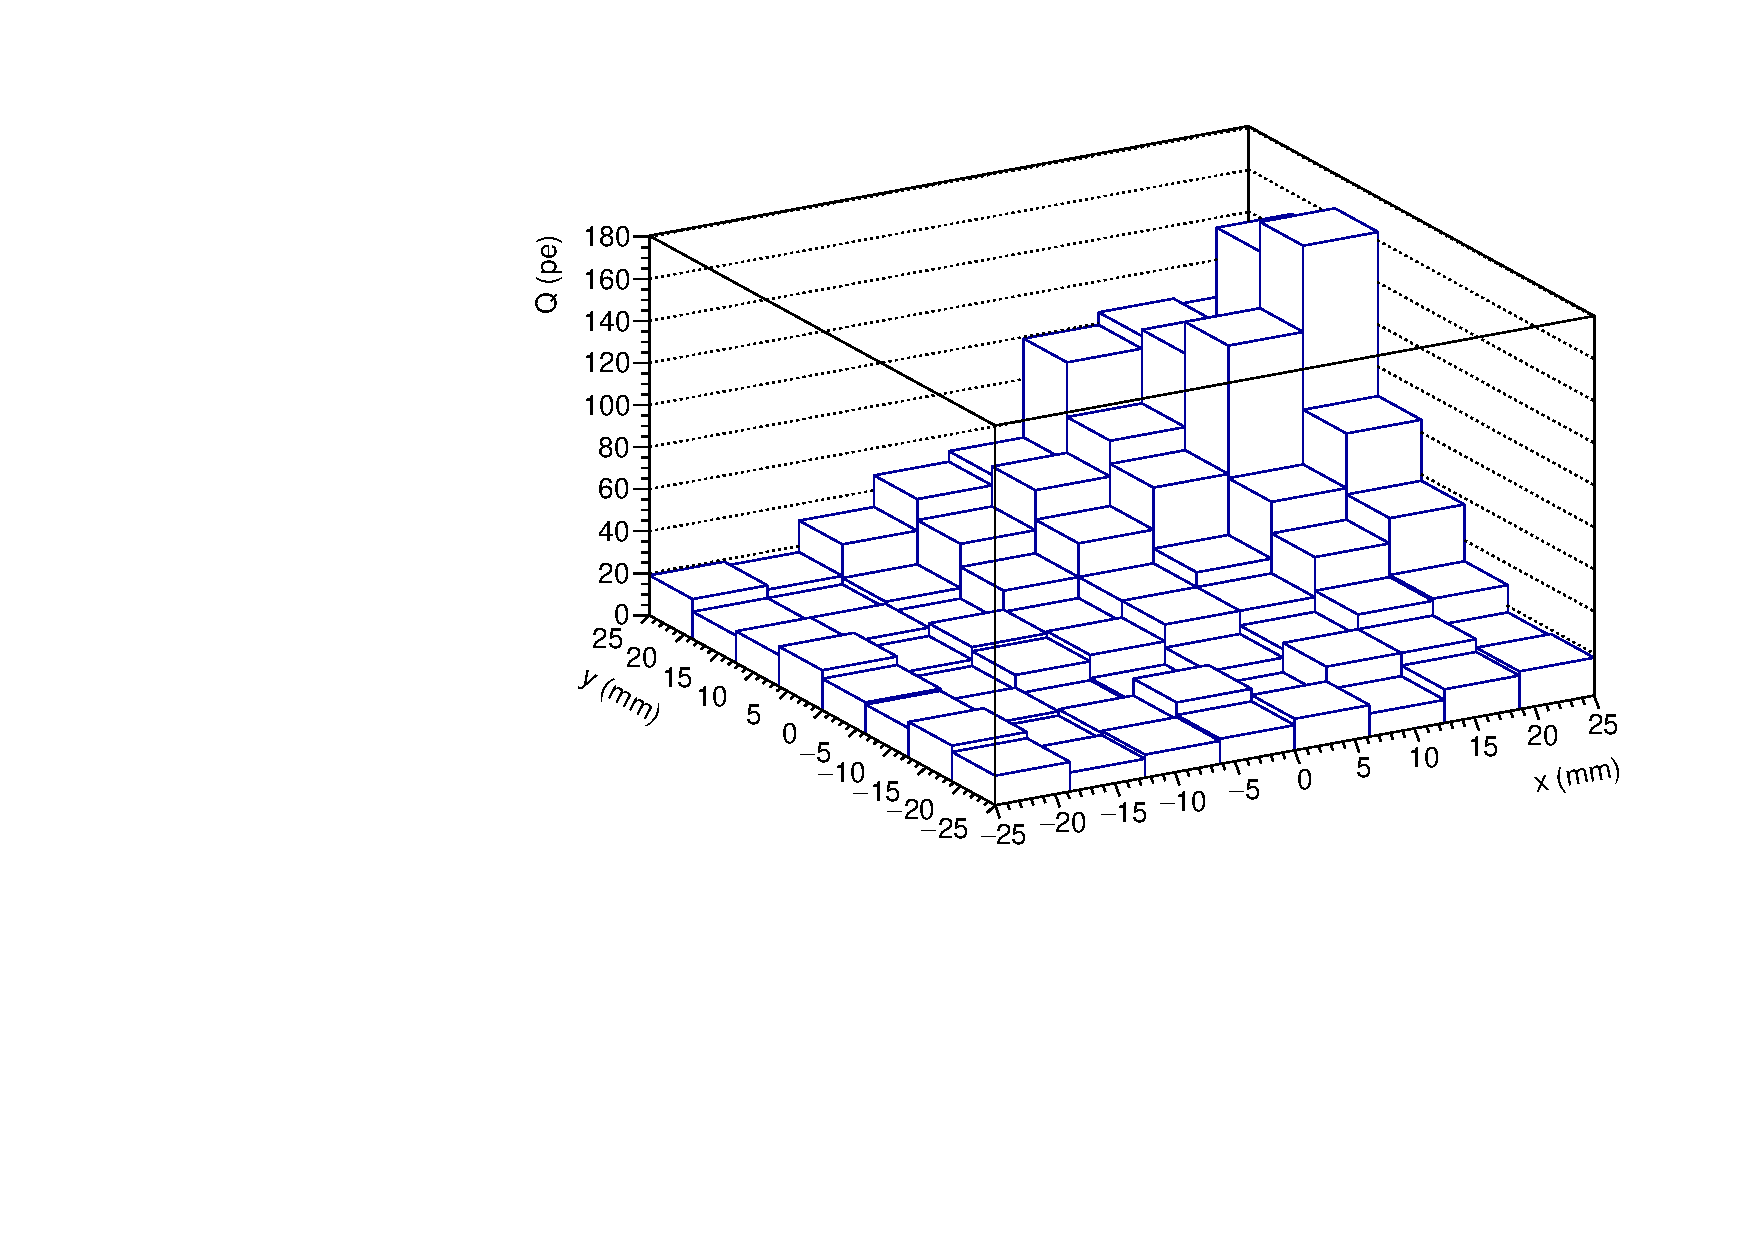
\includegraphics[width=.5\textwidth]{img/compton_1cluster.pdf}
		\label{fig.compton2}
	}
	\caption{\label{fig.compton} Compton events can show one or two clusters depending on the distance between interaction points. (a) Gamma interacting on (-5.91,0.90,-22.33) and on (15.85,4.29,-22.31). (b) Gamma interacting on (10.63,17.50,-15.90) and on (18.39,11.65,-6.91)
	}
\end{figure}

\newpage
The distance between interaction points in Compton events is very important as Figure \ref{fig.compton} shows. If they are separated enough then two clusters will appear (Fig. \ref{fig.compton1}), but if not there will be only one peak, maybe flatter than a photoelectric event (Fig. \ref{fig.compton2}). 

\begin{figure}[htb!]
        \begin{center}
                \subfloat[Photoelectric MSS]{
                        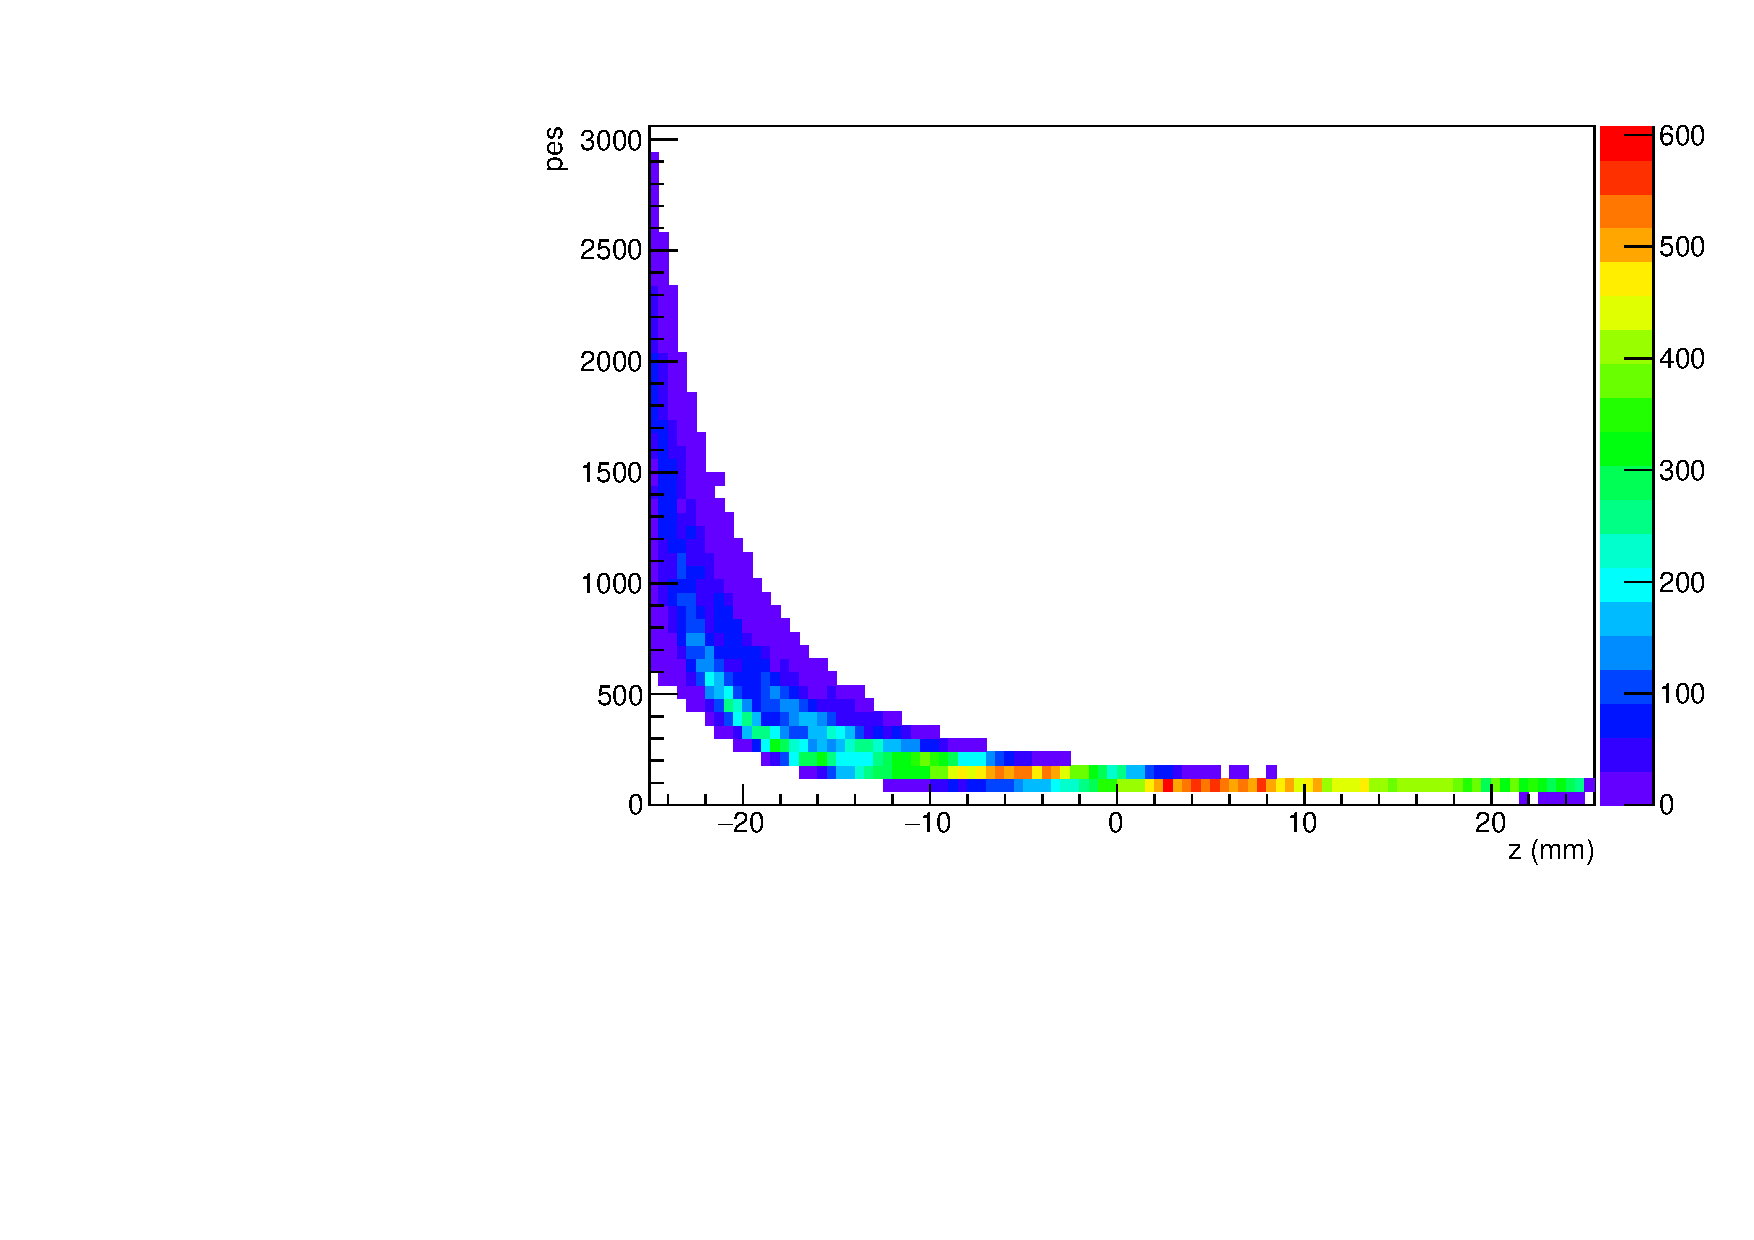
\includegraphics[width=.5\textwidth]{img/sipmmc_p0_2_z5.pdf}
                }
                \subfloat[Photoelectric 2nd MSS]{
                        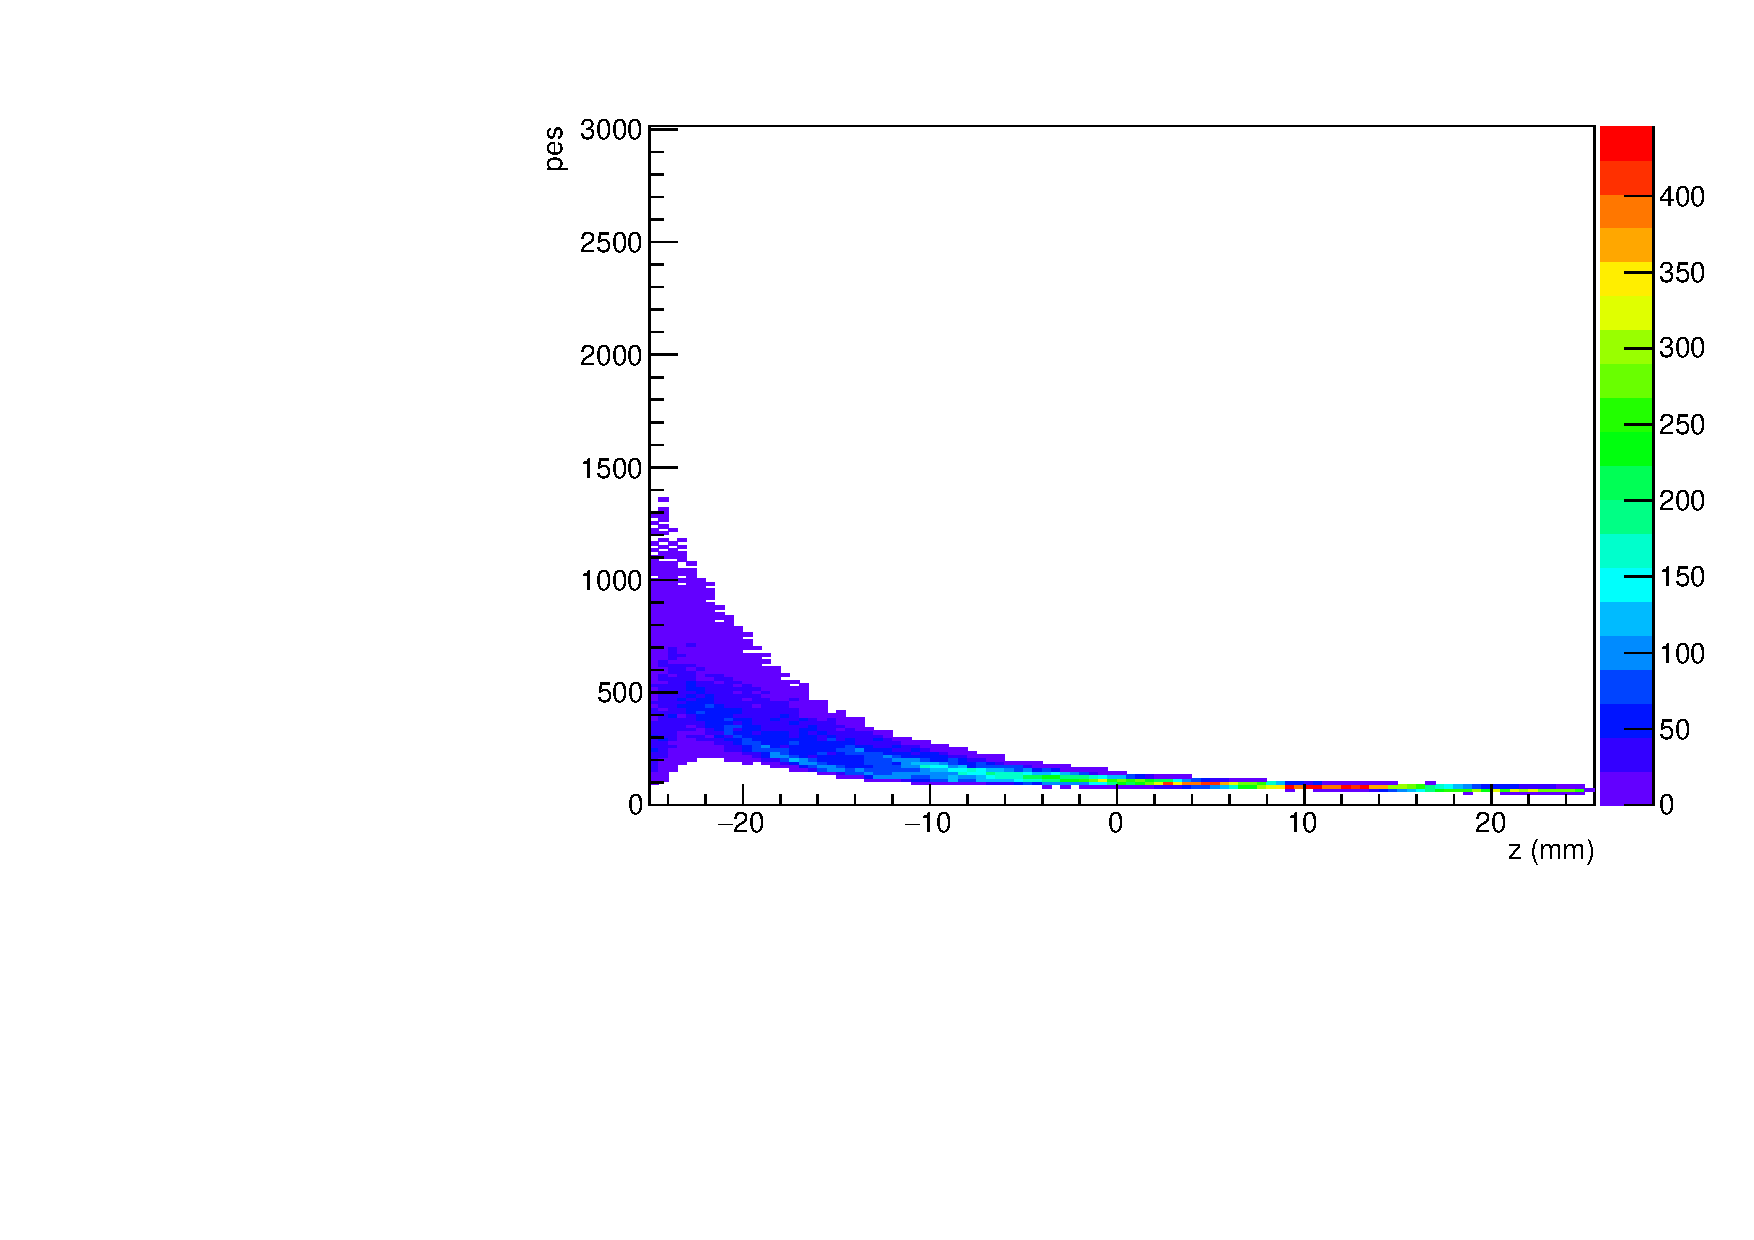
\includegraphics[width=.5\textwidth]{img/sipmmc_p0_2nd_2_z5.pdf}
                }\\[-2ex]
                \subfloat[Compton MSS]{
                        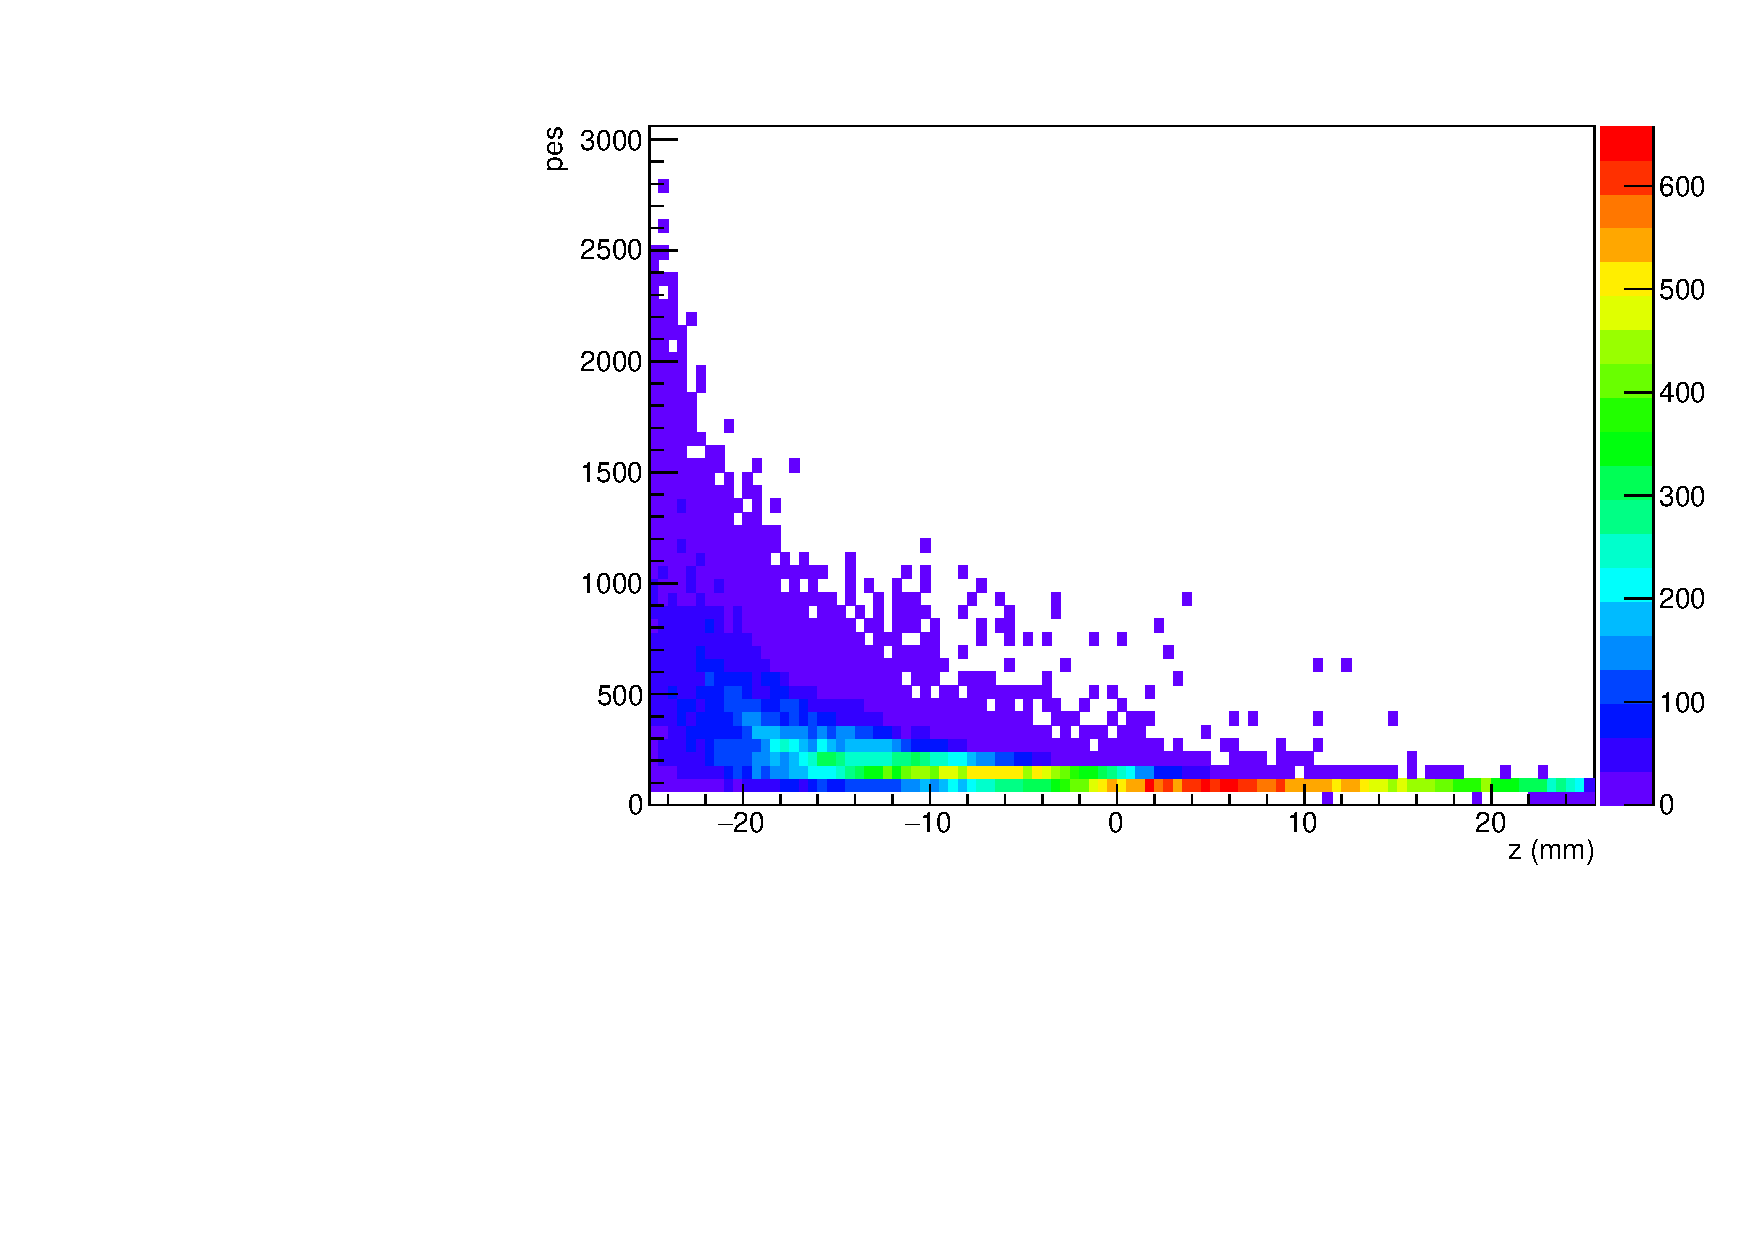
\includegraphics[width=.5\textwidth]{img/sipmmc_p0_compt_2_z5.pdf}
                }
                \subfloat[Compton 2nd MSS]{
                        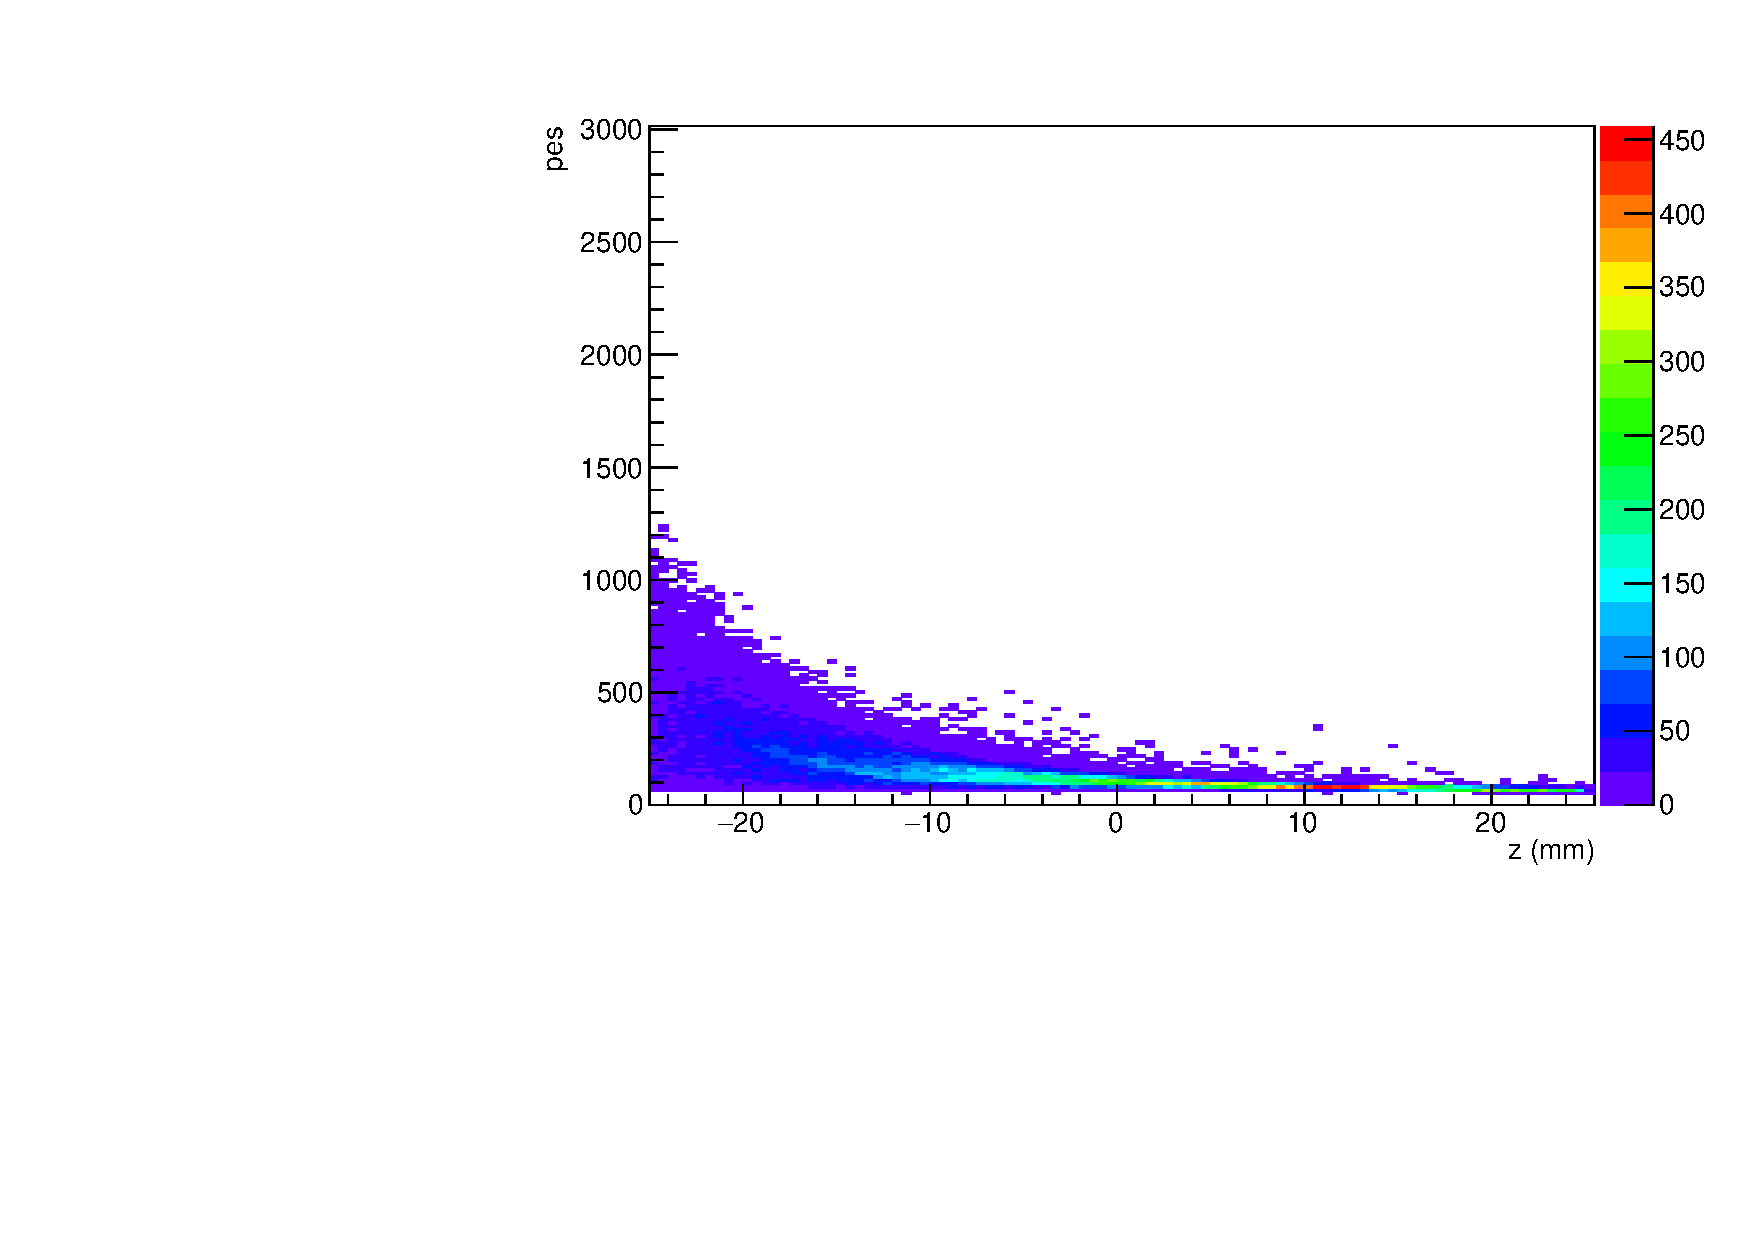
\includegraphics[width=.5\textwidth]{img/sipmmc_p0_2nd_compt_2_z5.pdf}
                }\\
                \caption{\label{fig.sipmmc} All plots shows charge registered on entry plane (at $z=-25$). (a) MSS charge for photoelectric events. (b) Charge of the new maximum after removing MSS for photoelectric events. (c) MSS charge for Compton events. (d) Charge of the new maximum after removing MSS for photoelectric events}
        \end{center}
\end{figure}


A criteria that allows us to discriminate between photoelectric and Compton events has to be defined. Compton events have more than one vertex and the total charge should be distributed among them. We can try to find this, for instance, looking at the SiPM with maximum signal (max signal sensor or MSS) and at the new maximum after removing MSS for photoelectric and Compton events. This is shown in Figure \ref{fig.sipmmc}, the upper histograms show the first and second MSS for photoelectric events and the lower ones the same for Compton events. It is clear that the charge of the second MSS is much smaller than the first in both types of events (beware of the scale). There are some differences but most events appear in the same places, making this criteria unsuitable for discriminating.

The same procedure can be done with the MSS and the first corona of SiPMs adjacent to it (MSS+C1). This is shown in Figure \ref{fig.sipmmcc1}. It can be seen that some Compton events have more charge in the second cluster than the photoelectric ones, but this is a minority. 

It is not clear yet how to solve this problem. One direction we want to explore is using neural networks receiving as input the values of all SiPM and training them to identify what kind of event it is (Compton or photoelectric).

\begin{figure}[h!]
        \begin{center}
                \subfloat[Photoelectric MSS+C1]{
                        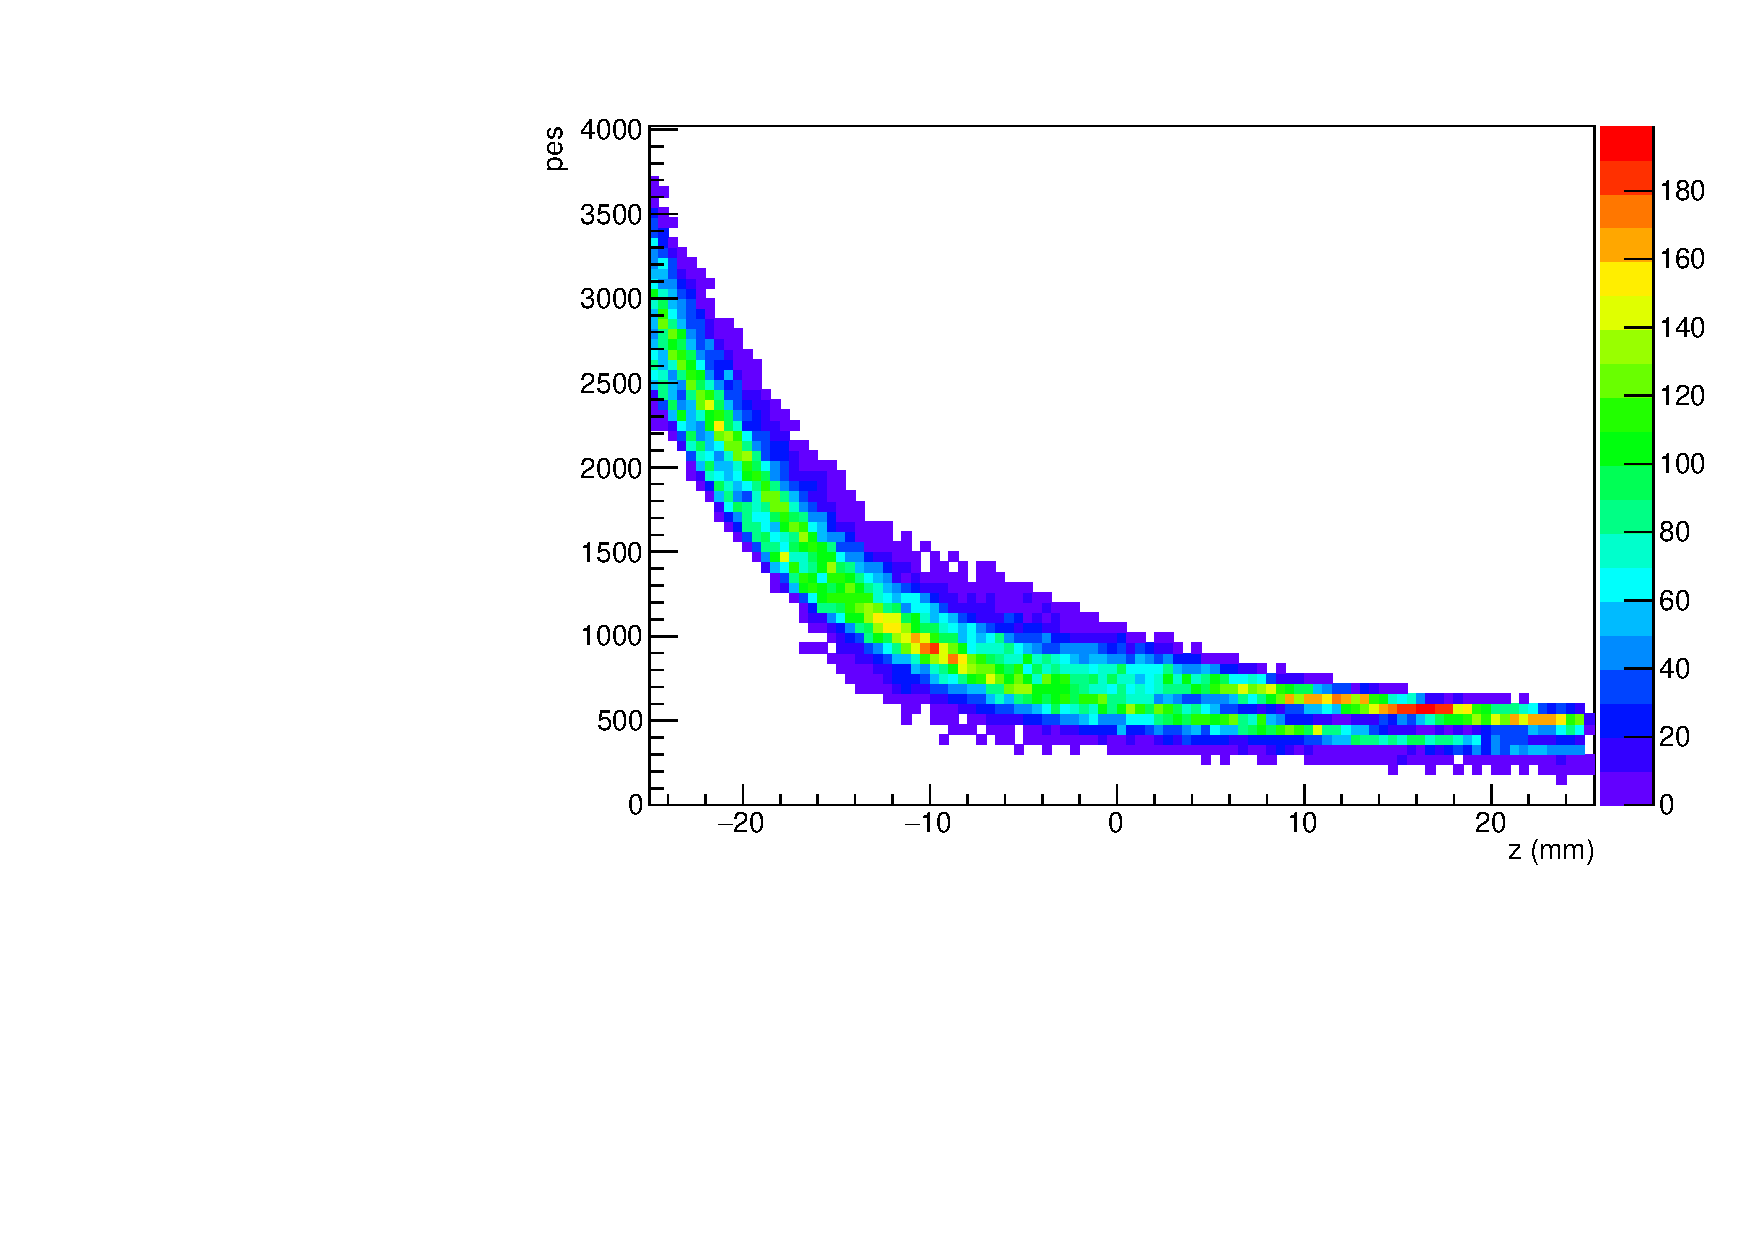
\includegraphics[width=.5\textwidth]{img/sipmmc_c1_p0_2_z5.pdf}
                }
                \subfloat[Photoelectric 2nd MSS+C1]{
                        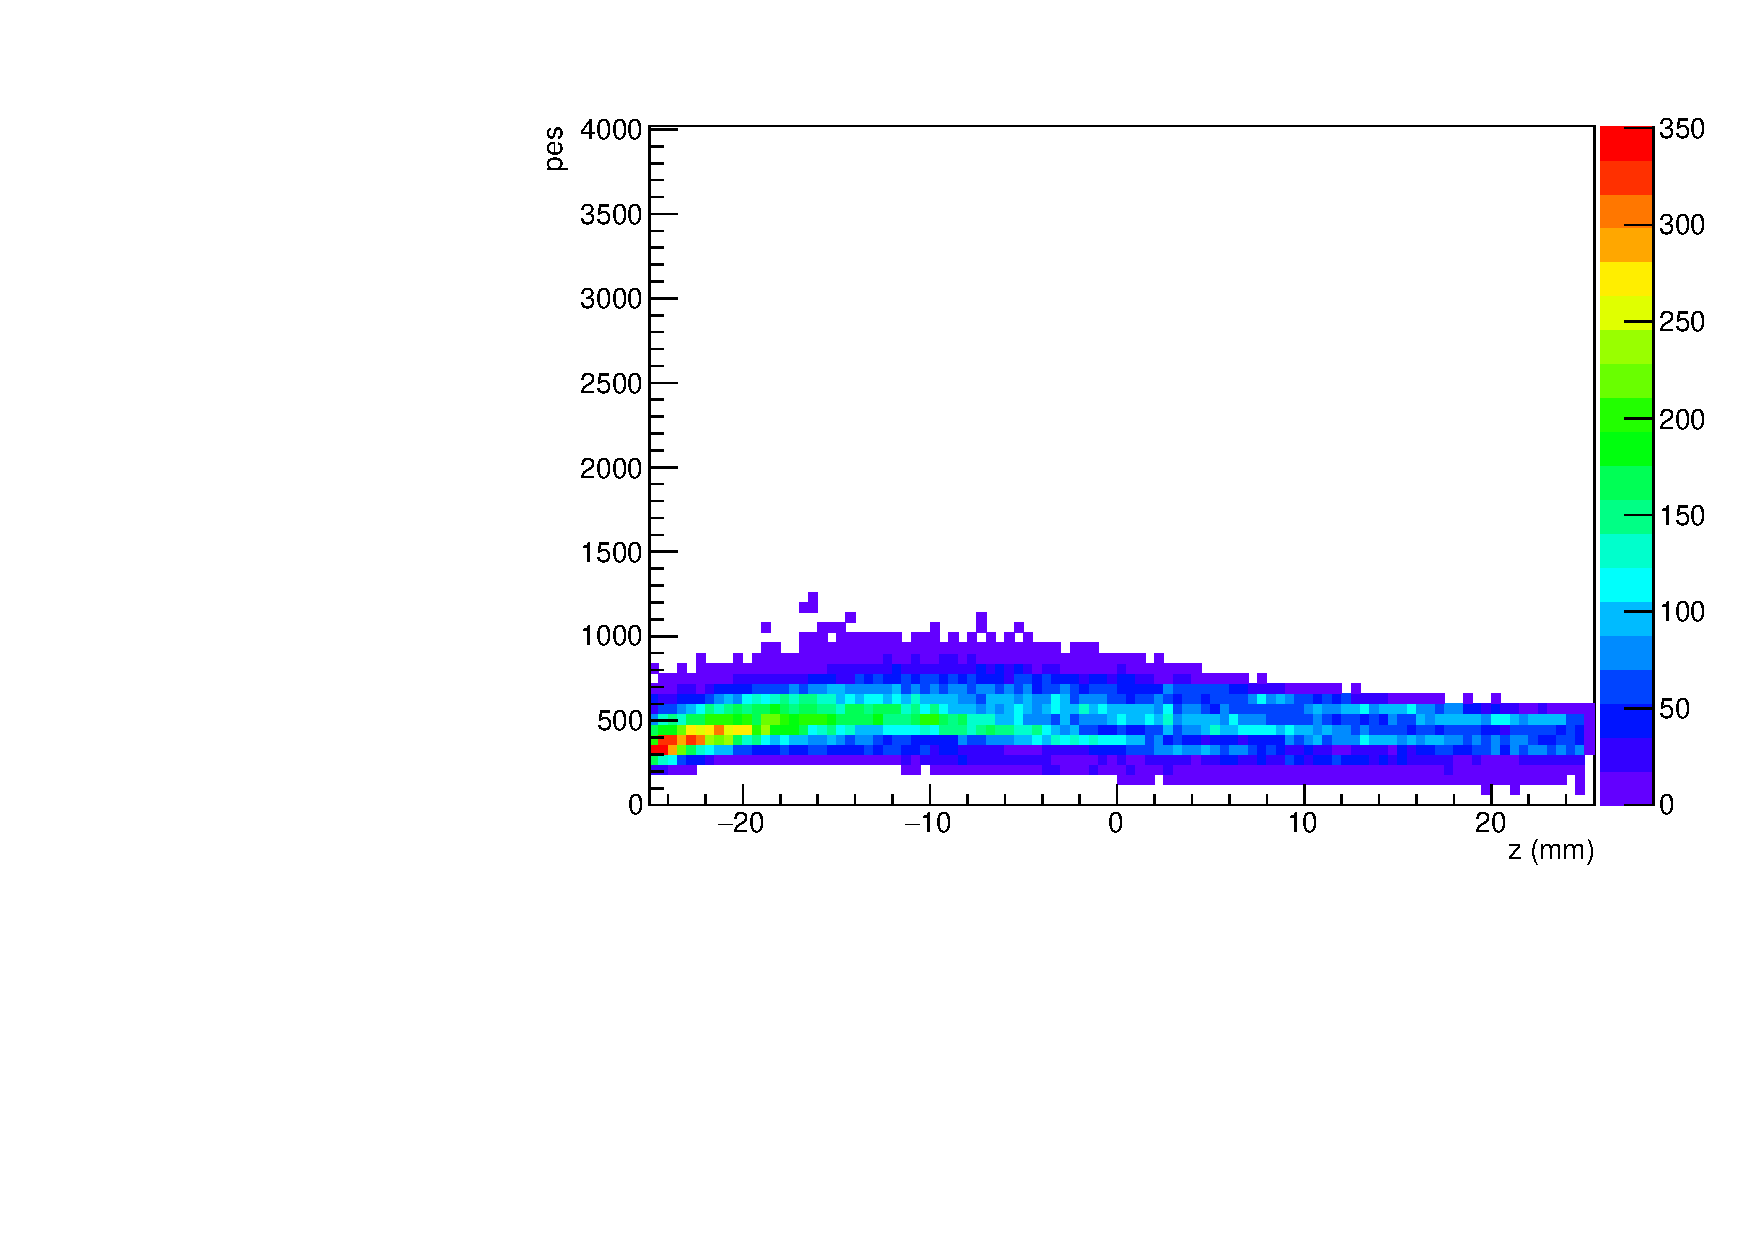
\includegraphics[width=.5\textwidth]{img/sipmmc_c1_p0_2nd_2_z5.pdf}
                }\\[-2ex]
                \subfloat[Compton MSS+C1]{
                        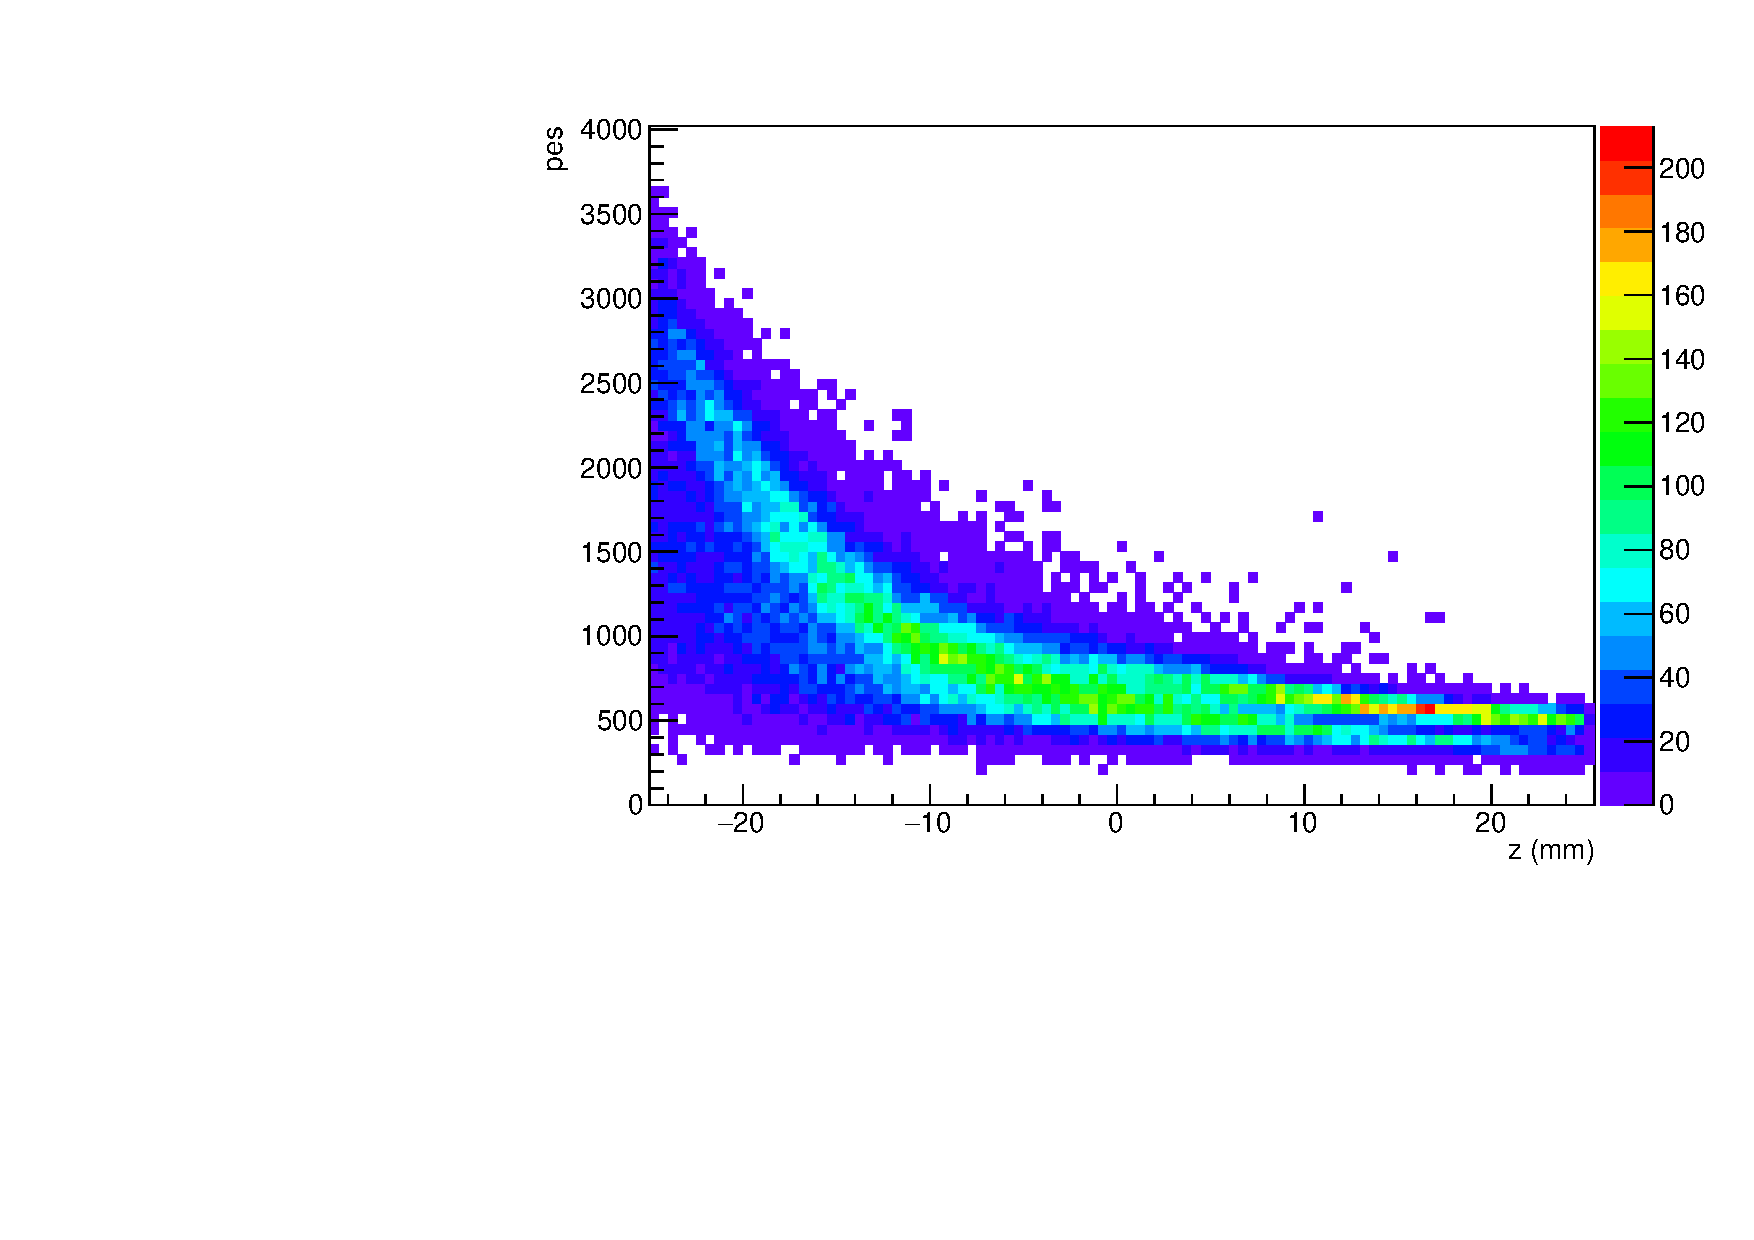
\includegraphics[width=.5\textwidth]{img/sipmmc_c1_p0_compt_2_z5.pdf}
                }
                \subfloat[Compton 2nd MSS+C1]{
                        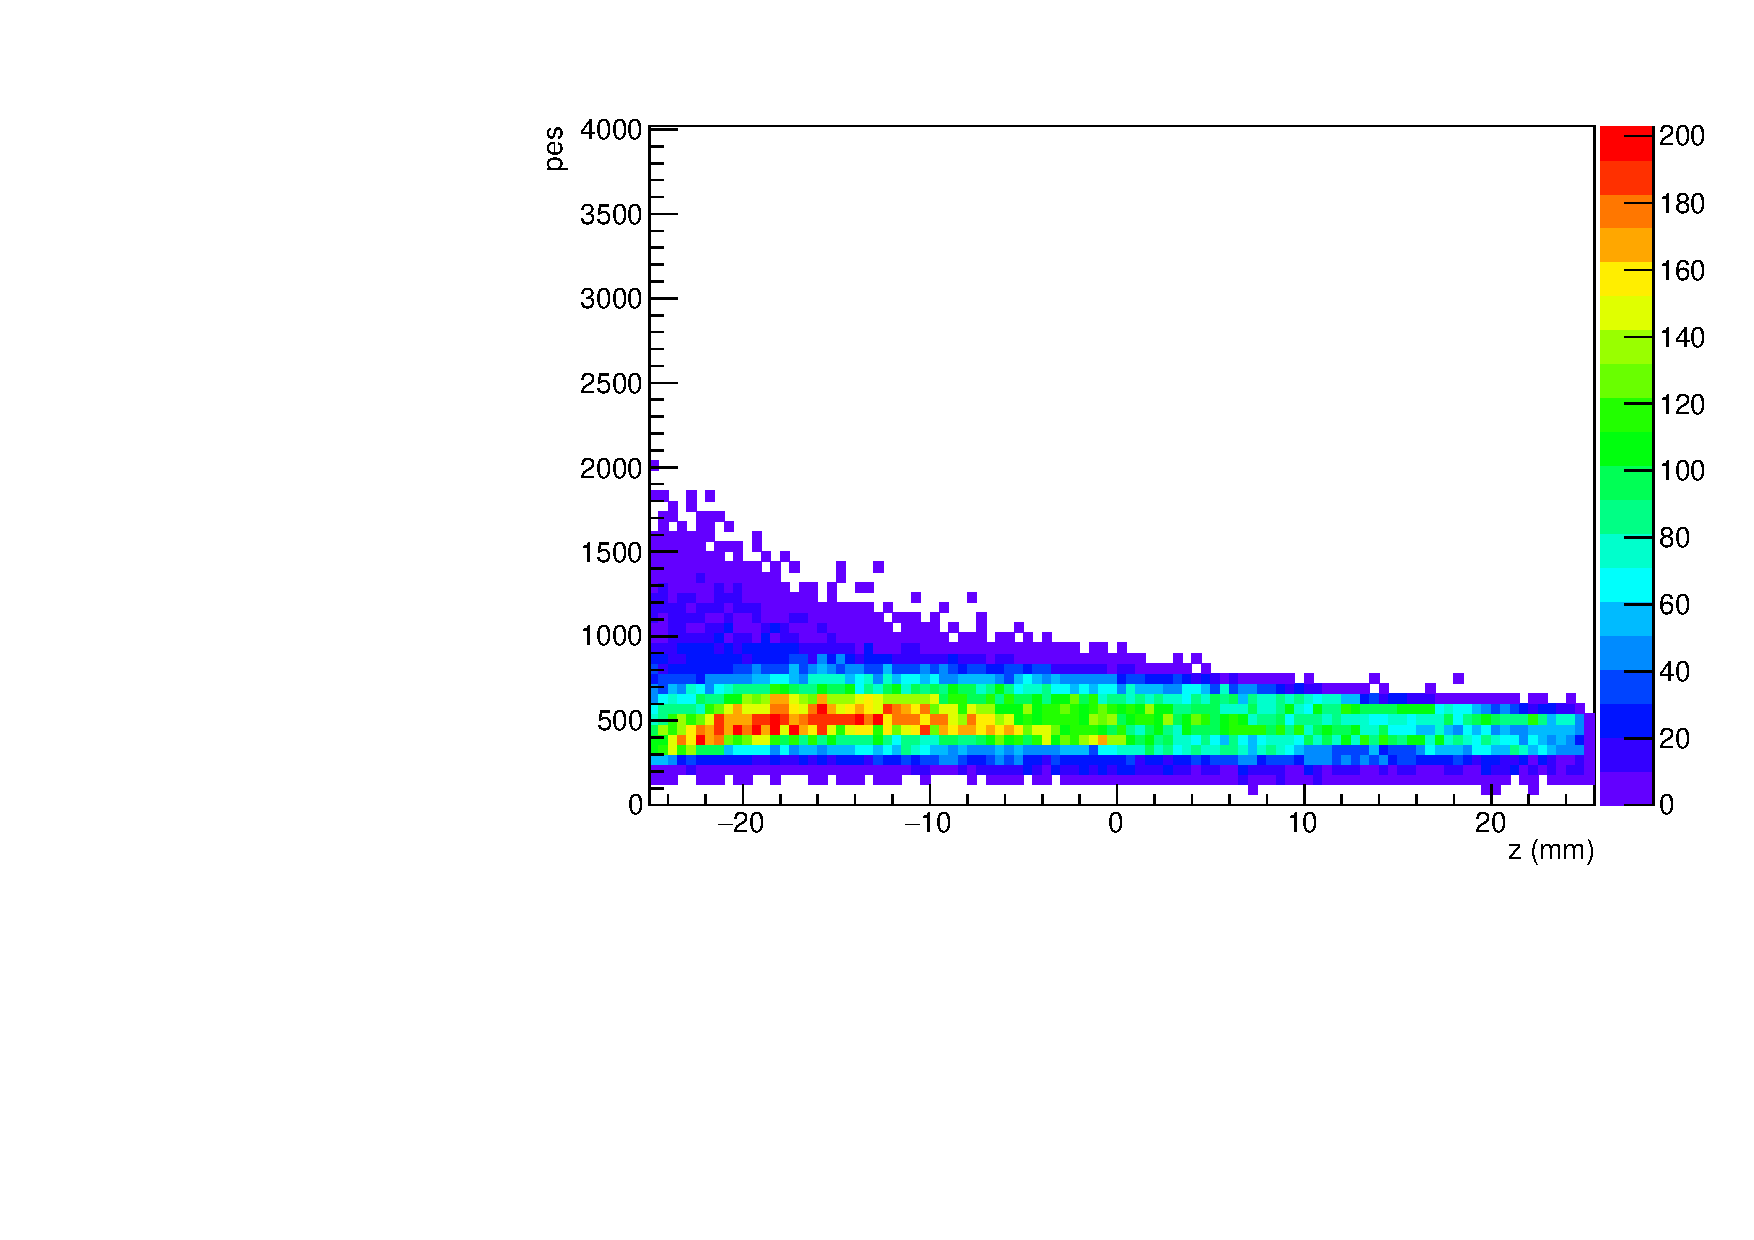
\includegraphics[width=.5\textwidth]{img/sipmmc_c1_p0_2nd_compt_2_z5.pdf}
                }\\
                \caption{\label{fig.sipmmcc1} All plots shows charge registered on entry plane (at $z=-25$). (a) MSS+C1 charge for photoelectric events. (b) Charge of the new maximum and its corona after removing MSS+C1 for photoelectric events. (c) MSS+C1 charge for Compton events. (d) Charge of the new maximum and its corona after removing MSS+C1 for Compton events.}
        \end{center}
\end{figure}
